\chapter{Experimental setup}\label{ch:belle2}

An important strategy to study \B meson decays is by dedicated colliders, known as $B$ factories.
$B$~factory experiments operate by producing large quantities of \BB pairs, through the creation of \FourS mesons that primarily decay to a \B meson pair (\BB) \cite{Workman:2022ynf}.
Historically, two $B$ factory experiments operated:
\begin{itemize}
    \item BaBar at the PEP-II accelerator at SLAC, USA \cite{BaBar:1995bns};
    \item Belle at the KEKB accelerator at KEK, Japan \cite{Belle:2000cnh}.
\end{itemize}
Another general flavour physics experiment is LHCb \cite{LHCb:2008vvz} with the LHC accelerator at CERN, 
collecting $B$ meson data produced in proton-proton collisions.
It has been operating since 2008.

Belle and BaBar are sometimes also referred to as first-generation asymmetric-energy $B$ factories, as they are the first that employed asymmetric beam collisions (see \Cref{sec:superkekb}).
CLEO \cite{CLEO:1982pvq} and ARGUS \cite{ARGUS:1988bds} experiments also collected significant $B$ meson datasets at symmetric \epem collision energy \FourS energies and are therefore sometimes considered predecessors to $B$ factories. 
An upgraded version of Belle, known as Belle~II, began collecting data in 2018.
Its main purpose is the collection of electron-positron (\epem) collision data 
at the centre of mass energies ($\sqrt{s}$) at or near the \FourS meson mass.
The colliding beams are provided by the SuperKEKB collider.
This chapter provides an overview of Belle II and introduces the main concepts of the SuperKEKB accelerator.

\section{The SuperKEKB accelerator}\label{sec:superkekb}

The SuperKEKB accelerator, discussed in detail in Ref.~\cite{Akai:2018mbz}, is a double-ring electron-positron collider.
It is an upgraded version of the KEKB collider \cite{Oide:2009zz} that operated with the Belle experiment, a predecessor to Belle~II.
The SuperKEKB accelerator complex is schematically shown in \Cref{fig:superkekb}.
A photo-cathode radio-frequency gun produces two electron beams.
The first beam is subsequently accelerated to 7~\gev by a linear accelerator into the electron ring.
On the other hand, positrons are created by directing the second electron beam to a tungsten target.
%, producing bremsstrahlung photons which create electron and positron pairs.
The positrons are singled out using the magnetic field and accelerated to 1.1~\gev, injected into the damping ring and, finally,
accelerated by the linear accelerator to 4~\gev before entering the main positron ring.
The subsequent collision occurs inside the Belle~II detector, where the electron and positron rings meet (see \Cref{sec:belle2}).
\begin{figure}[htbp!]
    \centering
    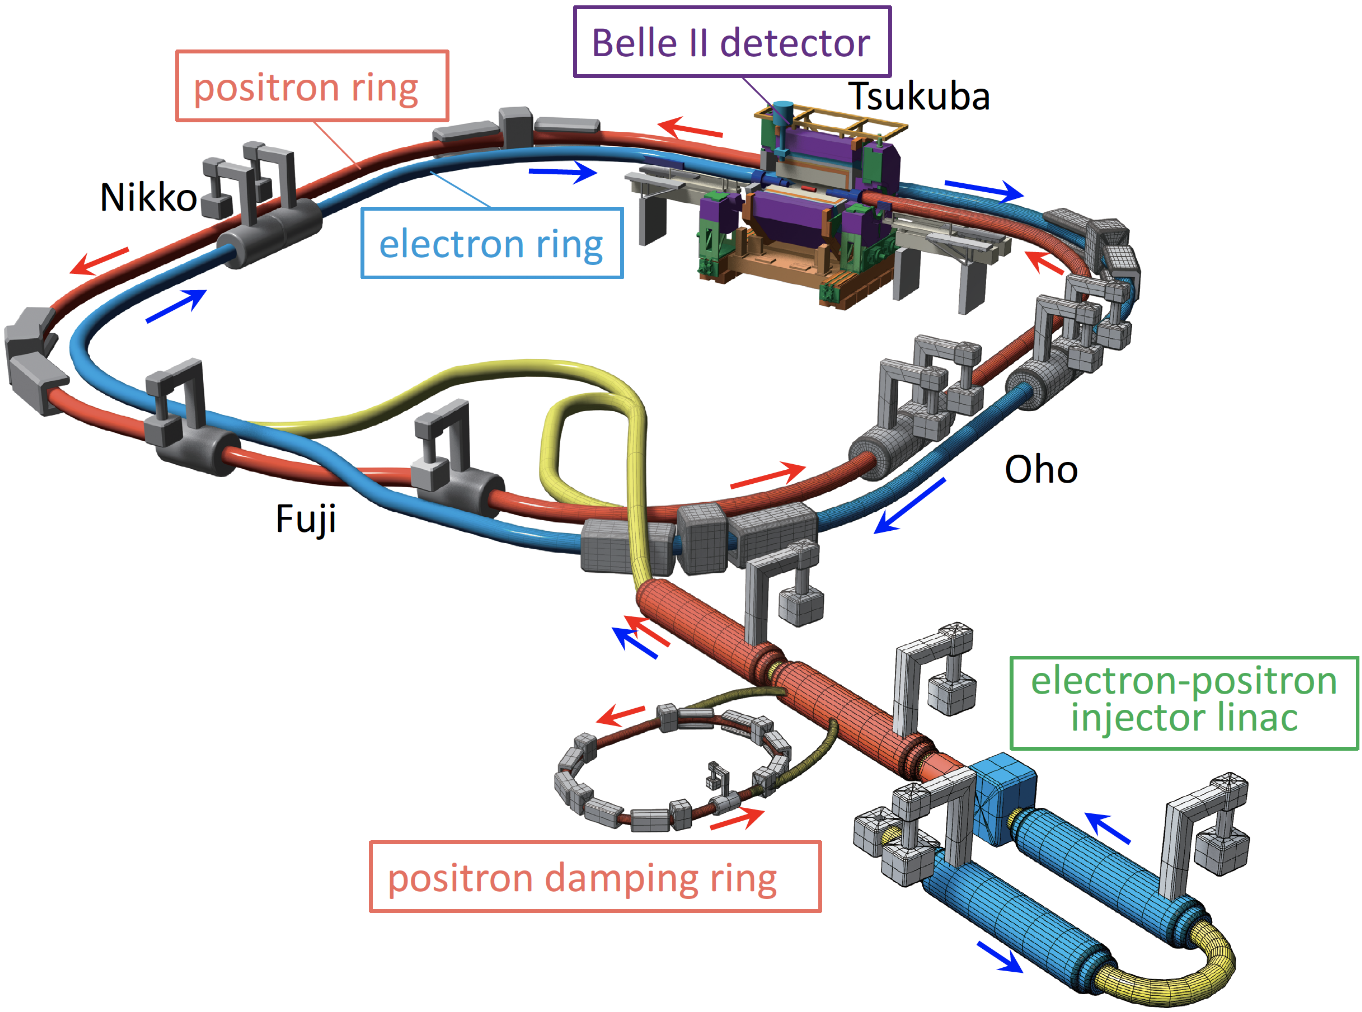
\includegraphics[width=0.6\textwidth]{figures/experimental_setup/super_kekb.png}
    \caption{\label{fig:superkekb}
        The schematic visualisation of the SuperKEKB accelerator complex.
        The main components that contribute to the acceleration of electrons and positrons are shown.
        The four straight sections are named after Japanese cities.
        Credit to Ref.~\cite{Akai:2018mbz}.
    }
\end{figure}

The beam-energy asymmetry (7~\gev for \en and 4~\gev for \ep) is an important design characteristic of SuperKEKB, 
which allows separating $B$ meson decay vertices by $\order(\si{\micro\meter})$, necessary for measurements such as time-dependent $\mathcal{CP}$ violation \cite{BaBar:2014omp}.
On the other hand, the exact collision energy is chosen to operate at $\sqrt{s}=\sqrt{(7+4)^2-(7-4)^2}~\gev\approx10.58~\gev$, which corresponds to the $m(\FourS)$, 
hence fulfilling the requirements of the $B$~factory experiment.

SuperKEKB also collects data at different $\sqrt{s}$.
For example, in the setup when the collision energy is lowered by 60~\mev, $\epem\ra\FourS$ events are not produced.
Such data, containing only low-multiplicity and continuum events, is called \textit{off-resonance} data.
Conversely, the conventional previously mentioned setup is referred to as \textit{on-resonance} data.

It is important to emphasise that an \epem collision at $10.58~\gev$ can produce more than just the \FourS.
Many other processes occur, such as $\epem\ra\ell^+\ell^-$ or $\epem\ra\qqbar$, and the production 
cross-section of all these processes depends on $\sqrt{s}$.
This is shown for $\sqrt{s}\approx10.58~\gev$ in \Cref{fig:cross_sections}, with more details about the exact values of the cross-sections provided in \Cref{sec:appendix_major_production_cross_sections}.
\begin{figure}[htbp!]
    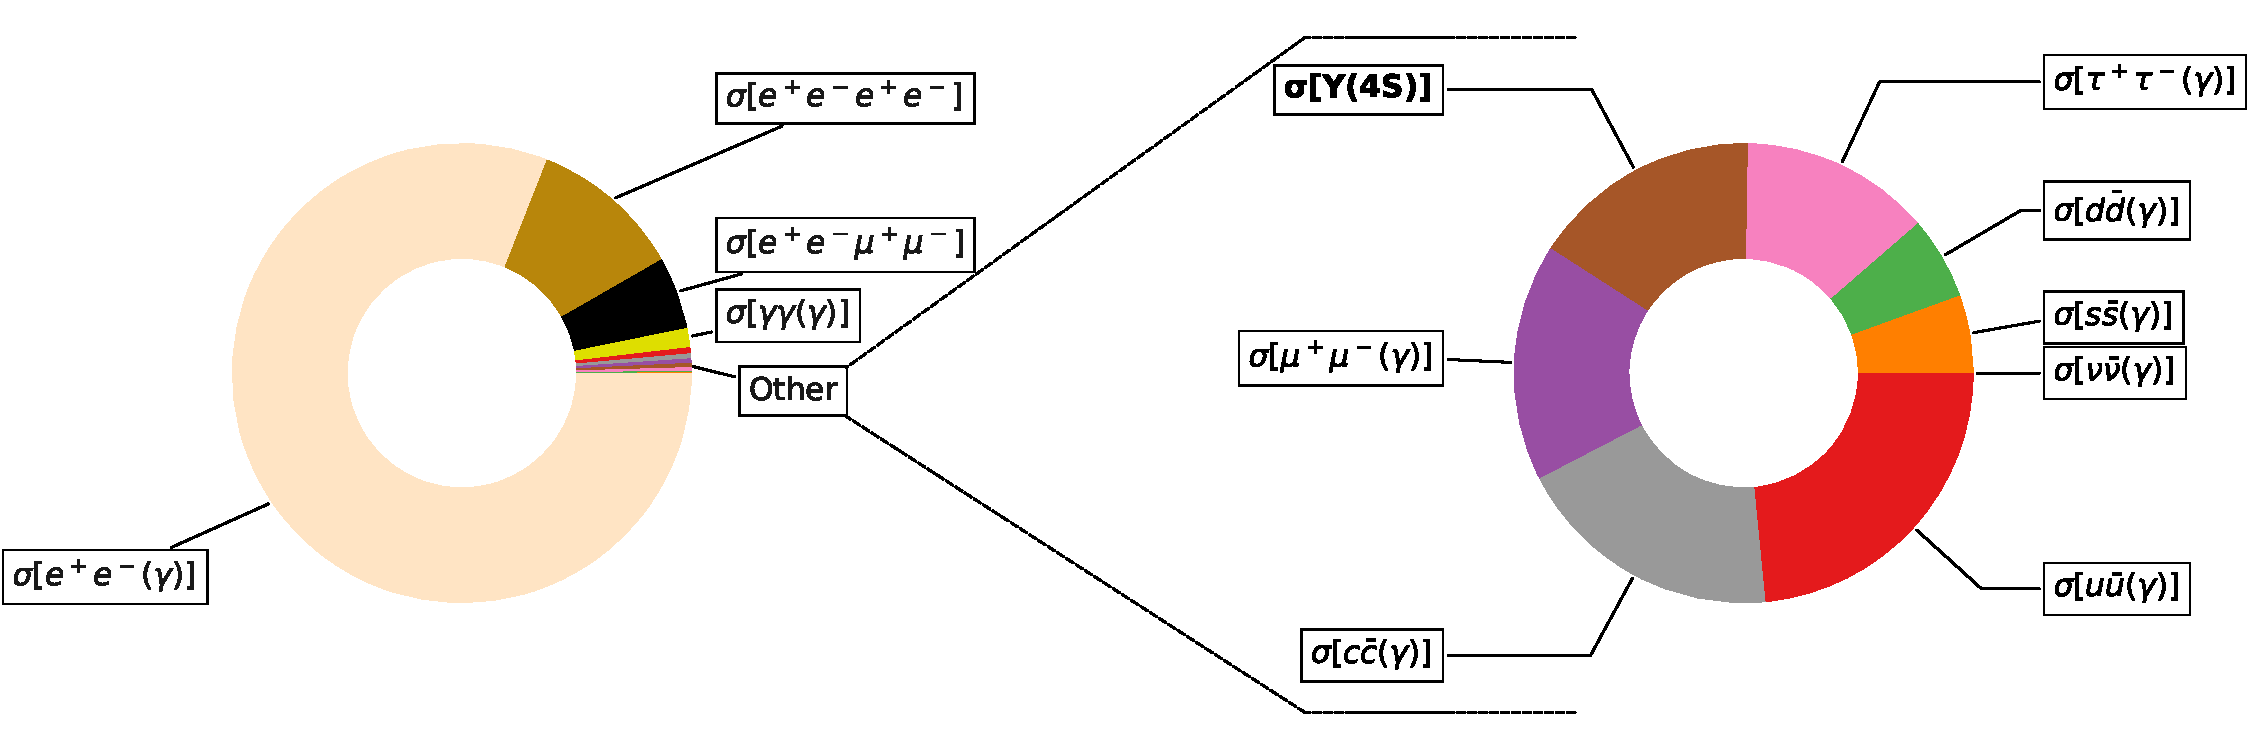
\includegraphics[width=1\textwidth]{figures/experimental_setup/corss_sections.pdf}
    \caption{\label{fig:cross_sections} Relative comparison of the largest $\epem\ra\ X$ production cross-sections at $B$~factories.
    The absolute scale of the cross-section is $\order(\nb^{-1})$.
    The exact numbers composing the charts are listed in \Cref{sec:appendix_major_production_cross_sections} and taken from \cite{Belle-II:2018jsg}.
    }
\end{figure}

Although by far the largest cross-sections are related to the \textit{low-multiplicity} processes, 
such as $\epem\ra\epem$ and $\epem\ra\mumu$ (see \Cref{sec:appendix_major_production_cross_sections}),
they differ largely from typical \FourS\ra\BB events.
On the other hand, the \textit{continuum} (\epem\ra\qqbar and \epem\ra\tautau) 
events are a significant background process for many analyses aiming to measure \B meson decays~\footnote{Because of the large $\epem\ra\qqbar$ and $\epem\ra\tautau$ production cross-sections, 
$B$ factories are also used to study charm mesons or $\tau^{\pm}$ and similar decays. 
In such cases, the continuum events are the events of interest.}.

SuperKEKB has a design luminosity of $L=8\times10^{35}\cm^{-2}s^{-1}$, which is 40 times higher than the maximum achieved by KEKB~\cite{Funakoshi:2022dai}.
Currently, SuperKEKB holds the instantaneous luminosity world record, which at the time of writing this thesis is $L = 4.65\times10^{34}\cm^{-2}s^-1$.
This is enabled by the increased beam intensity, upgraded beam focusing technique (nano-beam) and other improvements, which are beyond the scope of this thesis.


\section{The Belle II experiment}\label{sec:belle2}
The Belle II detector, discussed in detail in Ref.~\cite{Belle-II:2010dht}, is designed to reconstruct the final states of electron-positron.
Belle~II operates since 2018 and has collected 364~\invfb of on-resonance and 42~\invfb of off-resonance data by the time of writing this thesis.
The colliding beams are supplied by the SuperKEKB accelerator as discussed in~\Cref{sec:superkekb}.
The experiment is designed to collect 50~\invab of collision data, which will be nearly 50 times that of the combined datasets of all $B$ factories so far.
Belle II consists of several detector subsystems (\Crefrange{sec:pxd}{sec:klm}) arranged cylindrically around the beam pipe. 
The visual representation of the detector is given in \Cref{fig:belle2_detector} and shows the components of the detector with their acronyms.
\begin{figure}[htbp!]
    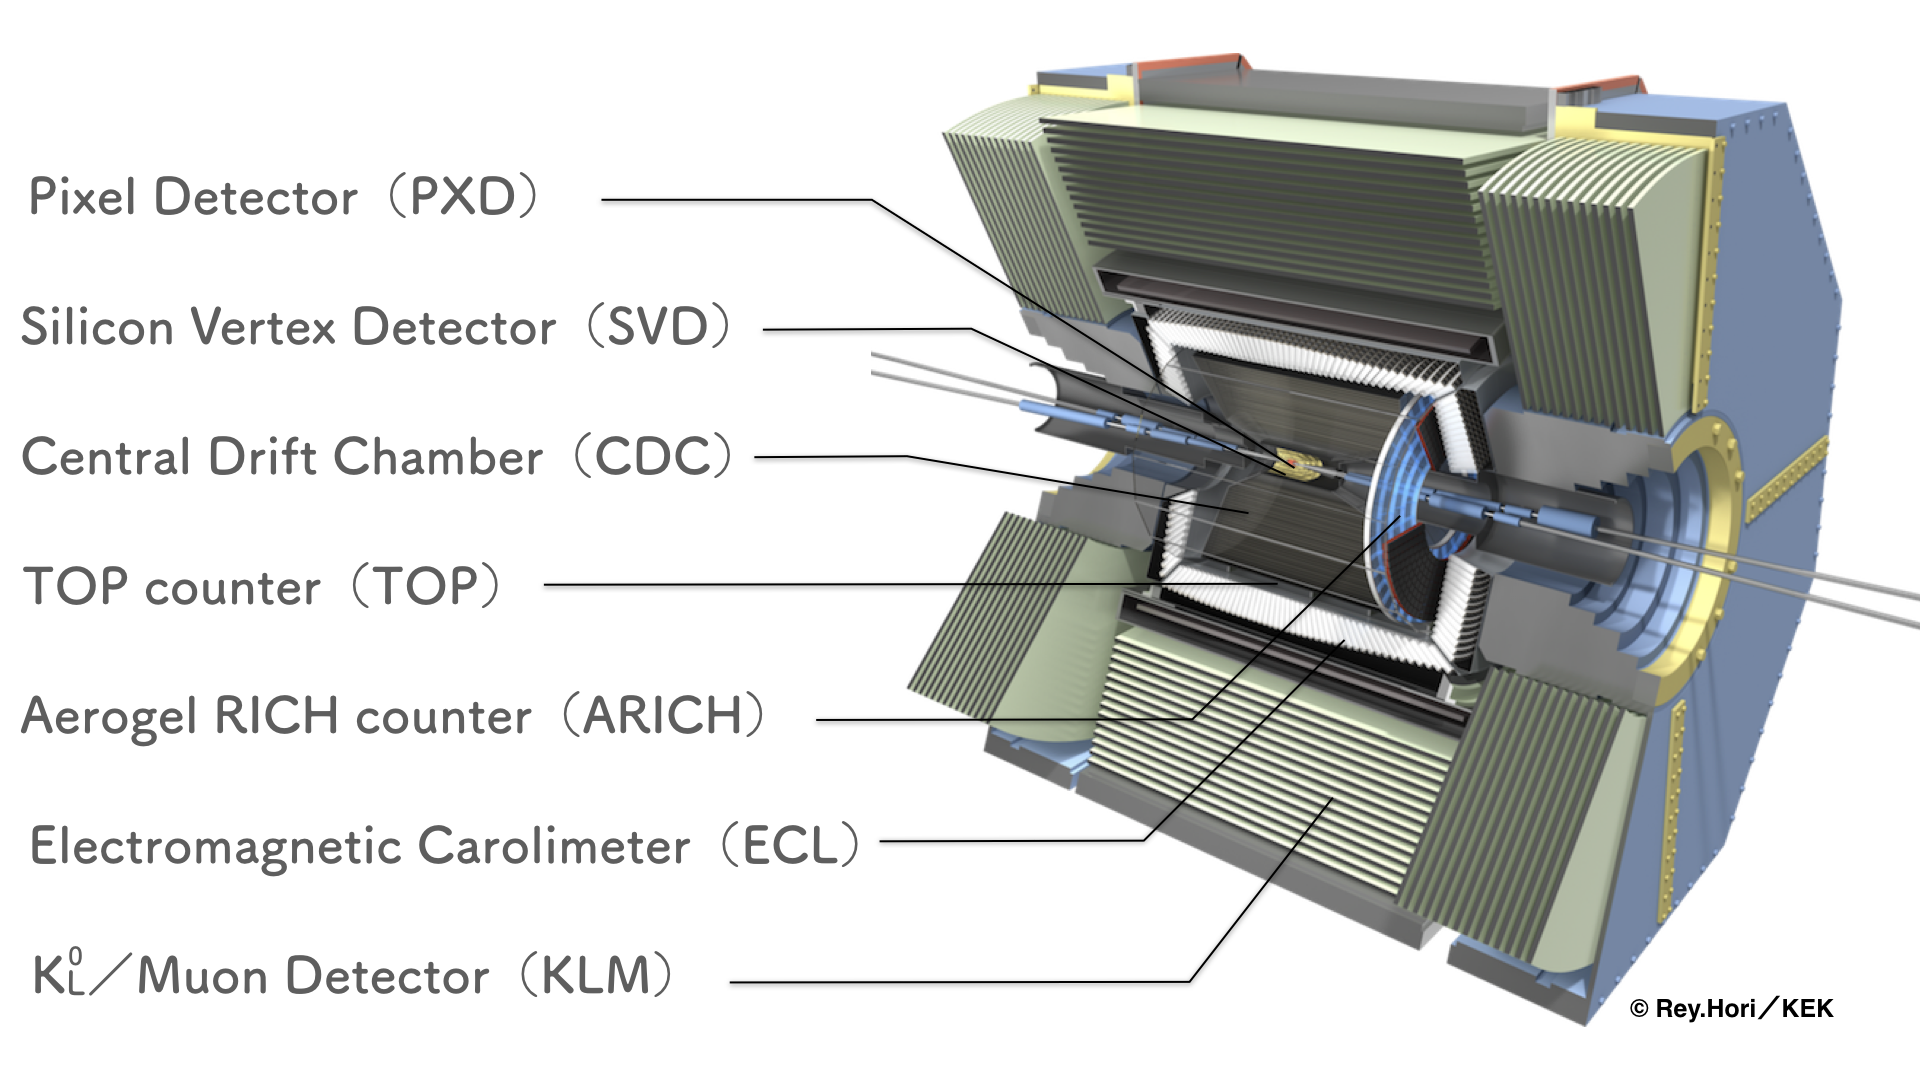
\includegraphics[width=1\textwidth]{figures/experimental_setup/belle2.png}
    \caption{\label{fig:belle2_detector} The schematic representation of the Belle~II detector.
    The Belle~II cylinder is approximately 7 meters in diameter and 7.5 meters long.
    The description of all sub-systems is provided in \Cref{sec:pxd,sec:svd,sec:cdc,sec:pid,sec:magnet,sec:ecl,sec:klm}.
    The Figure is taken from \cite{belle_2_picture}.
    Credit to the Belle~II collaboration.
    }
\end{figure}

\vspace{-12pt}
The coordinate system of Belle II is defined as follows: the $x$ axis is defined to be horizontal and points to the outside of the tunnel with respect to the accelerator's
main rings, the $y$ axis is vertically upward, and the $z$ axis is defined in the direction of the electron beam. 
The azimuthal angle, $\phi$, and the polar angle, $\theta$, are defined with respect to the $z$ axis. 
Three regions in the detector are defined based on $\theta$: 
\begin{itemize}
    \item forward endcap (\mbox{$12^{\circ}<\theta<31^{\circ}$}), 
    \item barrel (\mbox{$32^{\circ}<\theta<129^{\circ}$}),
    \item backward endcap (\mbox{$131^{\circ}<\theta<155^{\circ}$}).
\end{itemize}


\subsection{Pixel detector}\label{sec:pxd}

Closest to the collision point is the Belle~II Pixel Detector (\PXD)~\cite{Belle-II:2010dht}.
Its main purpose is the high-precision measurement of short-lived particle decay vertices, such as that of $B$ mesons.

The \PXD contains two layers of depleted $p$-channel field-effect transistors (\DEPFET) to detect charged particles that pass through it \cite{Kemmer:1986vh}.
The first layer is located at a 14~\mm radius from the collision point, whereas the second is at 22~\mm.
Each layer consists of 16 and 24 sensor modules, which are glued in pairs to make 8 and 12 ladders
\footnote{Until the scheduled 2023 Belle~II upgrade the outer layer contained only 2 ladders.}, respectively.
Each module contains $768\times250$ \DEPFET pixels.

The \PXD is designed to operate in large radiation conditions due to the proximity to the collision point,
while maintaining high-precision vertex reconstruction and a low material budget.
The sensors can withstand a $20~\si{\mega\radian}$ 
radiation dose and have a $\sim 0.2\%$ radiation length per layer \cite{Belle-II:2010dht},
while maintaining an average spatial resolution of approximately $15~\si{\micro\meter}$ and a hit efficiency of 99\% after 4 years of data taking \cite{Belle-IIDEPFET:2022wis}.
The subdetector is shown in \Cref{fig:pxd}, whereas its schematic location in the Belle~II detector is depicted in \Cref{fig:vxd}.

\begin{figure}[htbp!]
    \centering
    \subcaptionbox{\label{fig:pxd}}{
        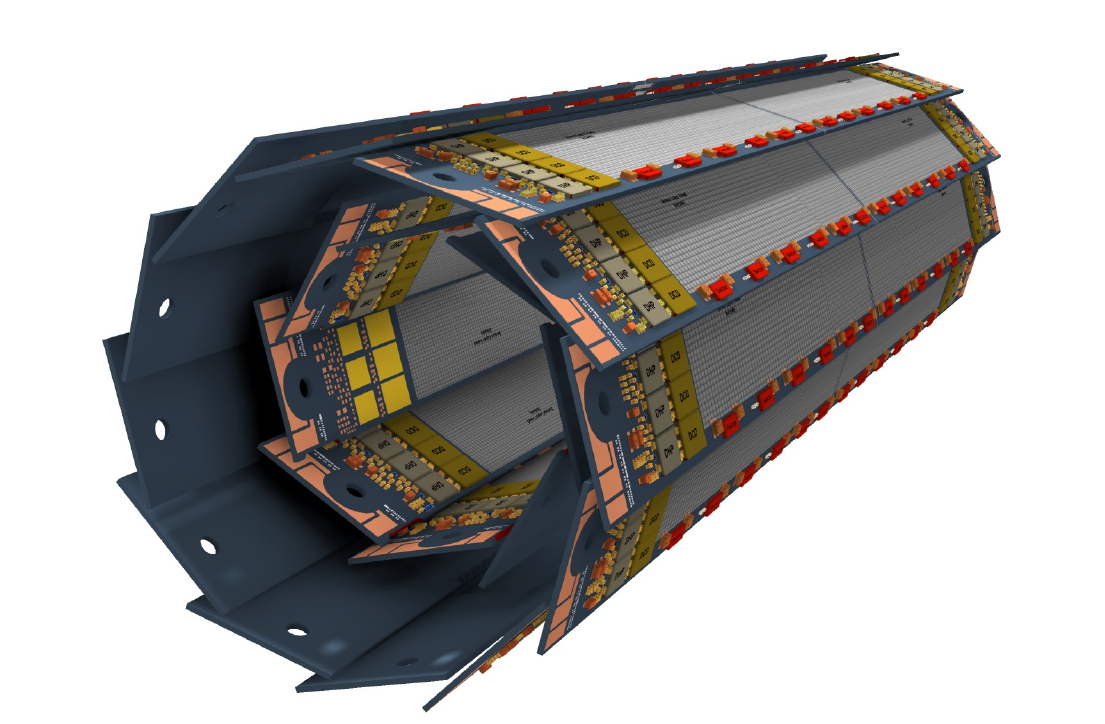
\includegraphics[width=0.45\textwidth]{figures/experimental_setup/pxd.png}
    }
    \subcaptionbox{\label{fig:svd}}{
        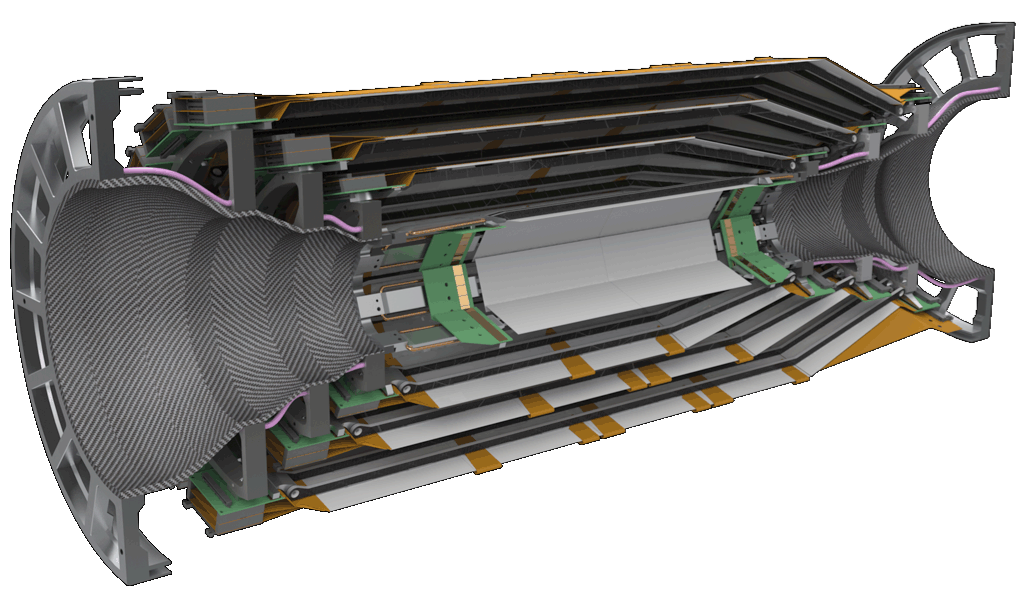
\includegraphics[width=0.45\textwidth]{figures/experimental_setup/svd.png}
    }
    \caption{\label{fig:pxd_svd} 
    The Belle II pixel (\Cref{fig:pxd}) and silicon vertex (\Cref{fig:svd}) detectors.
    They are installed in the Belle~II detector as shown in \Cref{fig:vxd}.
    The \PXD is arranged into two layers that are designed to contain 16 modules in the first layer and 24 in the second.
    The \SVD is composed of four layers around the \PXD, with a total of 172 double-sided silicon strip sensors.
    Credit to Belle~II PXD and SVD groups.}
\end{figure}

\subsection{Silicon vertex detector}\label{sec:svd}

The silicon vertex detector (\SVD) \cite{Belle-IISVD:2023mxk} surrounds the \PXD and 
is the second subsystem responsible for charged particle detection.
Its main roles include the reconstruction of short-lived particle decay vertices together with the \PXD,
standalone charged particle trajectory reconstruction for low momentum particles,
and particle identification through specific ionisation measurements.

The \SVD contains four layers. 
The first layer is composed of 7 ladders with 2 sensors,
the second of 10 ladders with 3 sensors,
the third of 12 ladders with 4 sensors,
and the final of 16 ladders with 5 sensors.
The 172 double-sided silicon strip sensors are composed, in total, of 224 000 strips.
Each sensor is based on an $n$-type bulk implanted with $p$ and $n$-doped sensitive strips.
The $p$ and $n$ strips are aligned perpendicularly and on opposite sides of the sensor.
The visual representation of the \SVD is shown in \Cref{fig:svd}, whereas its schematic location in the Belle~II detector is depicted in \Cref{fig:vxd}.

As charged particles pass through the \SVD sensors, the electrons and holes created through ionisation drift to $p$ and $n$ strips, respectively.
The perpendicularity of the strips ensures that the spatial coordinates of the passing particle can be inferred.

\begin{figure}[htbp!]
    \centering
    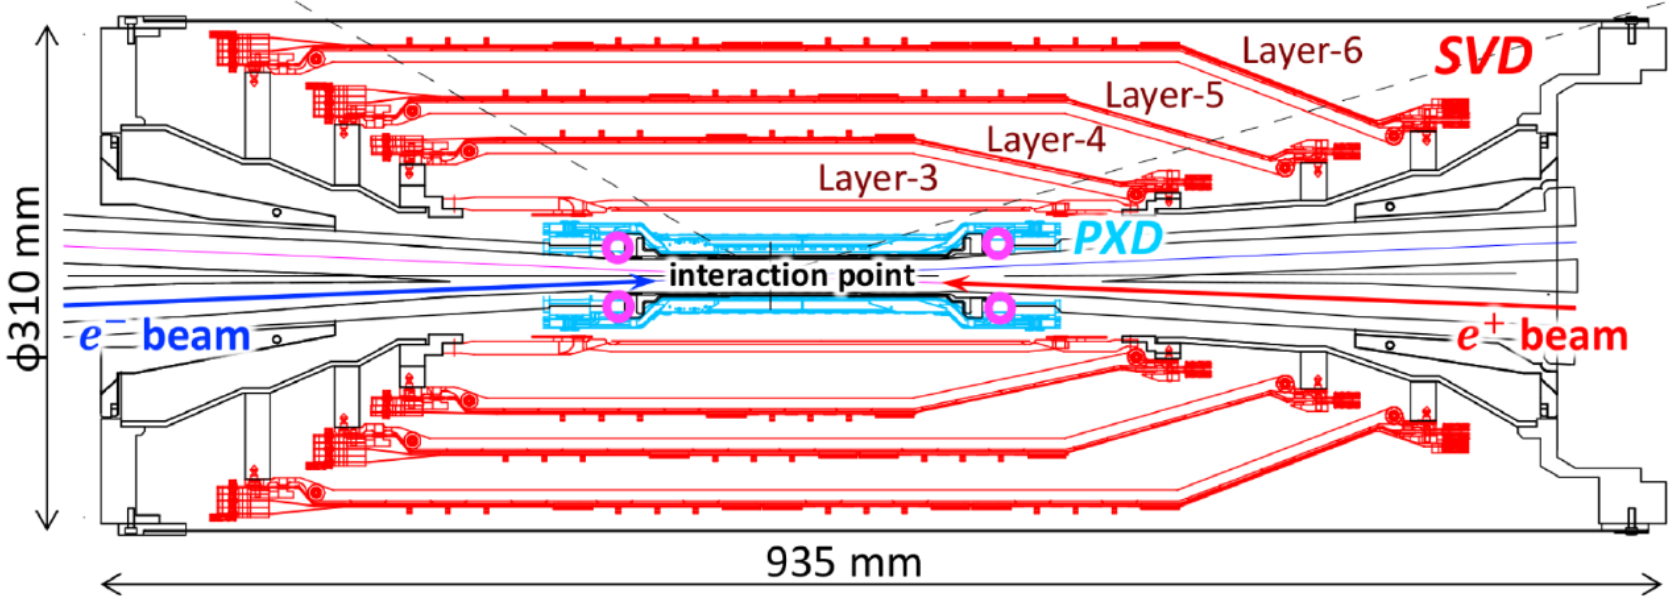
\includegraphics[width=0.6\textwidth]{figures/experimental_setup/vxd.png}
    \caption{\label{fig:vxd}
    The Belle II pixel and silicon vertex detectors are shown inside the Belle~II detector.
    The sizes of both vertex detection components and the interaction point location are noted.
    The Figure is taken from Ref.~\cite{Belle-IISVD:2023mxk}.
    }
\end{figure}

\subsection{Central Drift Chamber}\label{sec:cdc}

The central drift chamber (\CDC) \cite{Taniguchi:2017not} is the central subsystem responsible for the reconstruction of charged particle trajectories inside the Belle~II experiment.
As such, its main objective is the measurement of particle momenta and charge.
The \CDC also provides particle identification information through specific ionisation measurements
and participates in the decision to save the event information (\textit{triggering}).
It is a large volume drift chamber filled with a 50\% helium and 50\% ethane mixture.
The \CDC begins after the \SVD at $160~\mm$ and is contained within an outer cylinder radius of $1130~\mm$.
It consists of 14336 readout wires distributed across 56 layers.
Each readout is surrounded by 8 field wires that create an electric field in the chamber.
As a charged particle passes through the chamber ionising the gas,
the resulting electrons are accelerated in the electric field creating avalanches that are read out as signal by the wires.
In order to obtain three-dimensional information about the particle trajectory,
some layers in the \CDC are skewed.
The first 8 layers are axial, whereas the rest alternate between axial and skewed every 6 layers.
The grouping of layers is shown in \Cref{fig:cdc_quadrant}, whereas \Cref{fig:cdc_wires} illustrate the difference between axial ad skewed layers.

The \CDC covers $\theta\in(17,150)^{\circ}$ range and provides a highly accurate measurement of charged particle trajectories with a spatial resolution of $0.1-0.2~\cm$
and a transverse momentum resolution of $0.5\%$ for the majority of particles resulting from \B meson decays \cite{Kandra:2019qlz}.

\begin{figure}[htbp!]
    \centering
    \subcaptionbox{\label{fig:cdc_quadrant}}{
        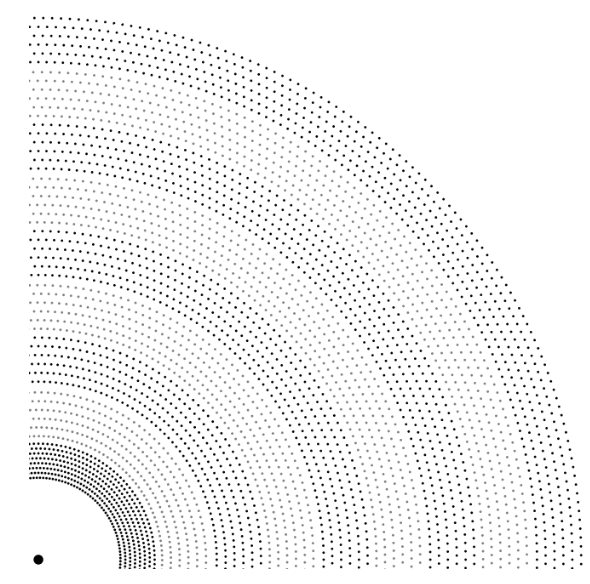
\includegraphics[width=0.45\textwidth]{figures/experimental_setup/cdc_quadrant.png}
    }
    \subcaptionbox{\label{fig:cdc_wires}}{
        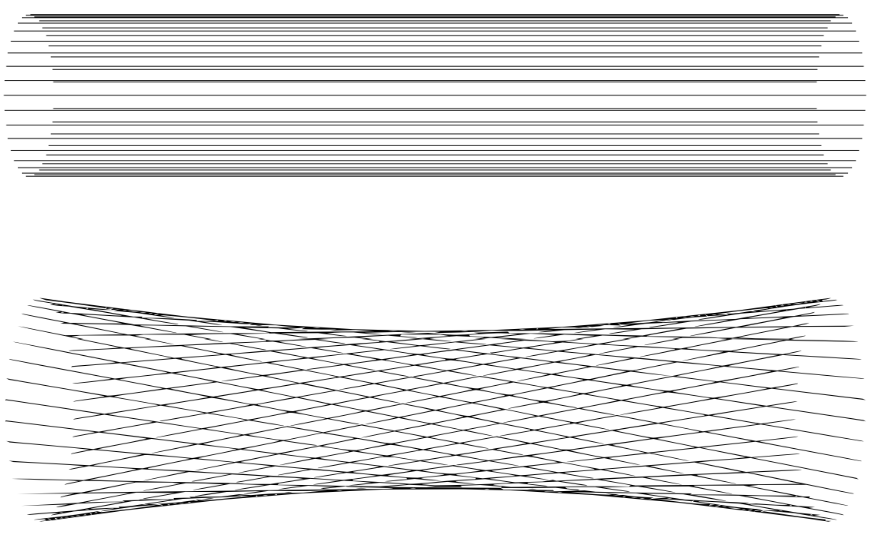
\includegraphics[width=0.45\textwidth]{figures/experimental_setup/cdc_layers.png}
    }
    \caption{\label{fig:cdc}
    The Belle~II central drift chamber schematic representation.
    \Cref{fig:cdc_quadrant} shows a quadrant of the \CDC in the $r$-$\phi$ plane.
    Different axial and skewed layer groups are visible.
    \Cref{fig:cdc_wires} shows the axial (upper) and (skewed) wires.
    The skew is exaggerated for illustrative purposes.
    Credit to Ref.~\cite{BelleIITrackingGroup:2020hpx}.
    }
\end{figure}

\subsection{Particle identification systems}\label{sec:pid}

Belle~II has two dedicated particle identification systems: an aerogel ring imaging Cherenkov counter (\ARICH) in the forward endcap region
and a time of propagation (\TOP) chamber in the barrel region. 
Both detectors are located outside the \CDC and are tasked with the distinction between particle species.

The \ARICH detector \cite{Yusa:2014tua} consists of an array of silica aerogel used as a radiator.
As charged particles pass through the material at a speed greater than the phase velocity of light in that medium, 
they emit Cherenkov photons, which are detected by photon sensors.
This working principle is depicted in \Cref{fig:arich}.
The angle of the emitted Cherenkov light, $\theta_C$, can be used to calculate its velocity, $\beta$, 
given the refractive index of the radiator material, $n$:
\begin{equation}
    \beta = \frac{1}{n\cdot\theta_C}.
\end{equation}
The velocity information, combined with the knowledge of the particle's momentum from the \CDC, \SVD and \PXD allows identifying the species of a particle through its mass.
\ARICH is designed to provide separation information for $\pi^{\pm}$ and $K^{\pm}$ in $(0.4,4)~\gevc$ momentum range, and for $\pi^{\pm},\mu^{\pm},e^{\pm}$ below 1~\gevc.

\begin{figure}[htbp!]
    \centering
    \subcaptionbox{\label{fig:arich}}{
        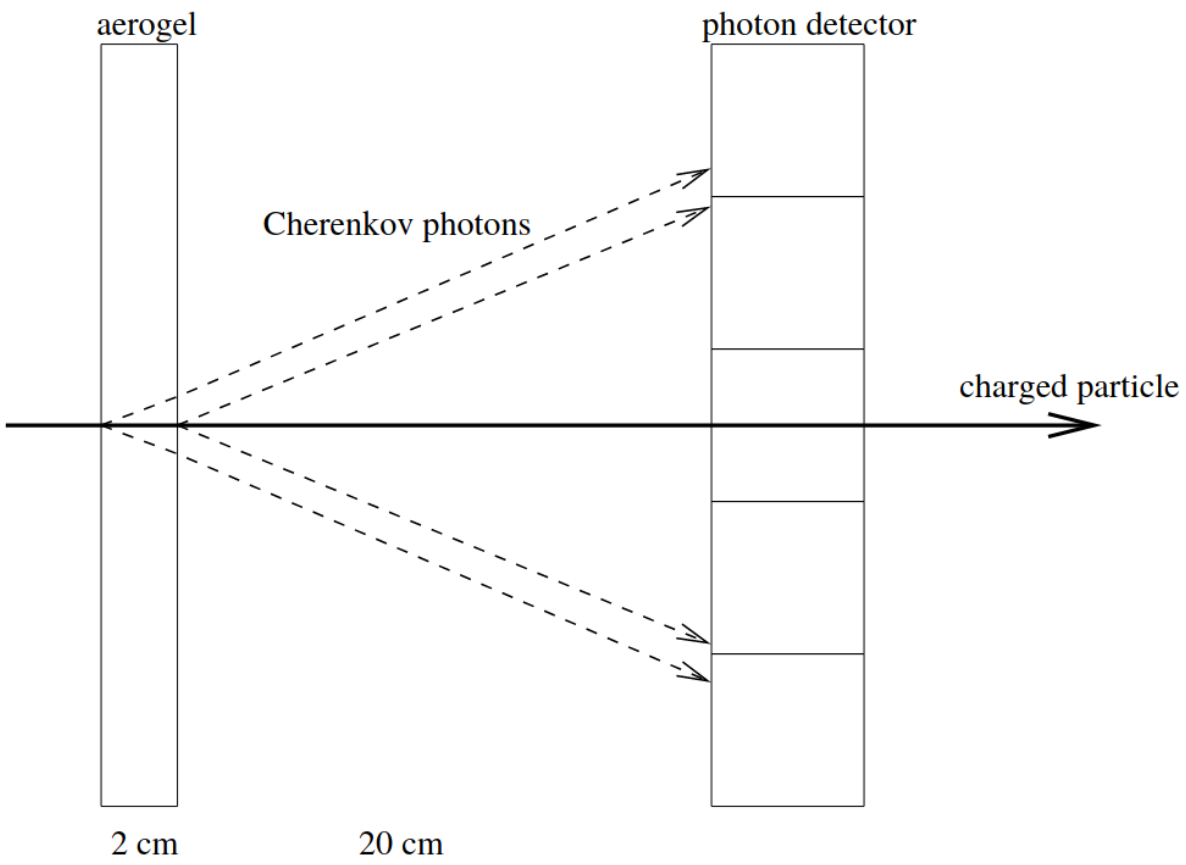
\includegraphics[width=0.4\textwidth]{figures/experimental_setup/arich.png}
    }
    \subcaptionbox{\label{fig:top}}{
        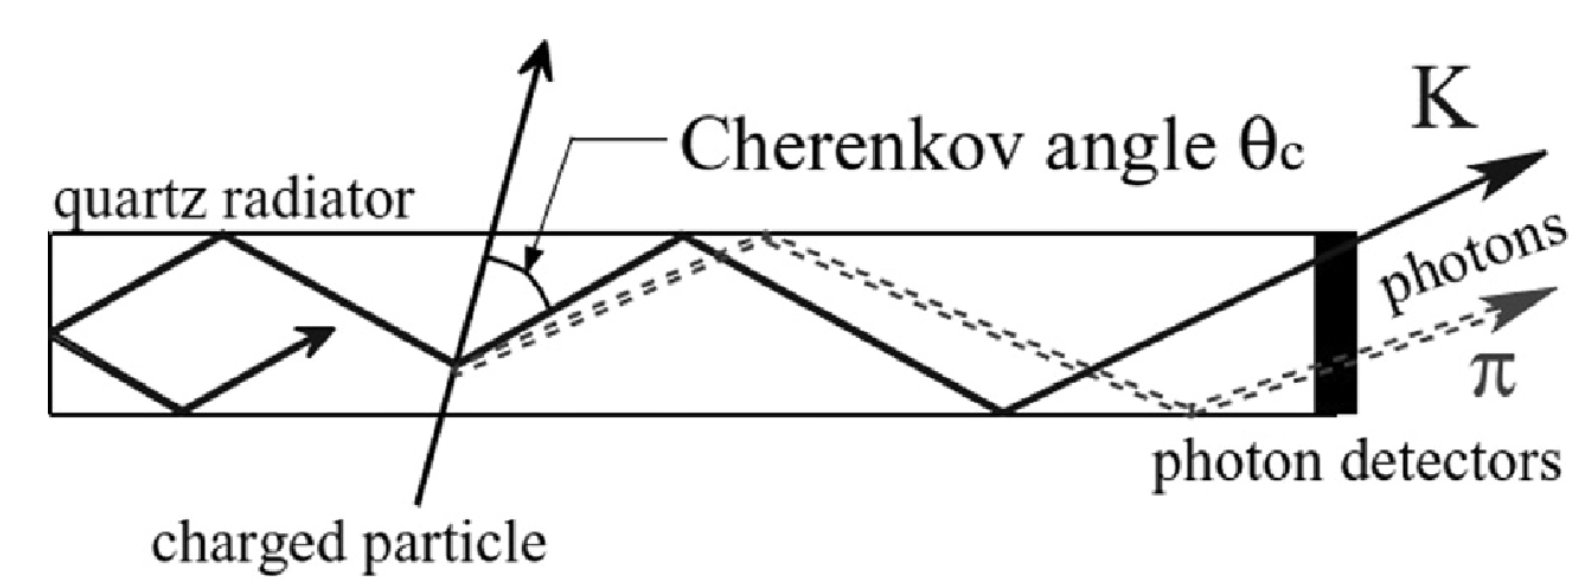
\includegraphics[width=0.45\textwidth]{figures/experimental_setup/top.png}
    }
    \caption{\label{fig:pid}
    The schematic working principle of the Belle~II particle identification detectors: aerogel ring-imaging Cherenkov counter (\Cref{fig:arich}) and a time of propagation chamber.
    \ARICH covers the forward endcap region, whereas \TOP covers the barrel.
    Credit to Refs.~\cite{Yusa:2014tua} and \cite{Fast:2017pff}, respectively.
    }
\end{figure}

The \TOP detector \cite{Fast:2017pff} consists of sixteen $270 \times 45 \times 2$~\cm quartz radiator bars.
The working principle is illustrated in \Cref{fig:top}.
One end of the quartz crystal contains a spherical mirror that reflects the light to the opposite end containing microchannel plate photomultiplier tube arrays.
The photon time of arrival is the sum of the time of flight of
the charged particle to the quartz radiator and the time of propagation
Due to the high refractive index of quartz, the Cherenkov light emitted by passing particles undergoes total internal reflection.
As a result, it propagates to the microchannel plate photomultiplier tubes. 
Given a precisely known angle of the incoming particle, the time of propagation inside the chamber is a function of~$\theta_C$.
The time of arrival of the photons is compared to the expected distributions for different particle hypotheses ($e^{\pm},\mu^{\pm},\pi^{\pm},K^{\pm},p^{\pm}$) and corresponding likelihood values are computed for each (see Ref.~\cite{Yonenaga:2020eby} for details).

The \TOP provides an 85\% identification efficiency for $K^{\pm}$ at a 10\% $\pi^{\pm}$ misidentification rate \cite{Kojima:2022qcl}.
The \ARICH has a 94\% efficiency for $K^{\pm}$ identification with a $\pi^{\pm}$ misidentification rate of 11\% \cite{Yonenaga:2020eby}.

\subsection{Electromagnetic calorimeter}\label{sec:ecl}

Belle~II reuses the calorimeter of Belle, with upgraded readout electronics \cite{Belle-II:2010dht}.
The electromagnetic calorimeter (\ECL) surrounds the previously mentioned detector systems and covers the barrel and both endcap regions.
It is the main subdetector for photon detection and energy measurements.
Furthermore, the \ECL provides information necessary to differentiate electrons from hadrons, participates in $K_L^0$ detection together with \KLM,
supplies triggering information, and measures the luminosity collected by the detector.

The \ECL covers $\theta\in(12.4,155.1)^{\circ}$ and is composed of 8736 thalium-doped caesium iodide crystals \cite{Miyabayashi:2020xzp}.
Each crystal is approximately 16 radiation lengths long \cite{Aulchenko:2015nvy}.
The rear surfaces of the crystals contain glued photodiodes with preamplifiers.
As electromagnetically interacting particles pass through the calorimeter, they induce cascades of particles through interaction with the dense detector material, called electromagnetic showers.
The photodiodes read out the scintillation light of the shower and convert it to a digital signal.
The sketch of a single \ECL crystal is given in \Cref{fig:ecl}.

The \ECL has excellent performance: a photon energy resolution which varies from 4~\% at 100~\mev \cite{Miyabayashi:2020xzp} to 2~\% at 5~\gev \cite{Aulchenko:2015nvy},
a position resolution of $5-10~\mm$ \cite{Miyabayashi:2020xzp}, and a mass-resolution of 5~\mevcc(12~\mevcc) for the composite \piz ($\eta$) meson \cite{Miyabayashi:2020xzp}.

\begin{figure}[htbp!]
    \centering
    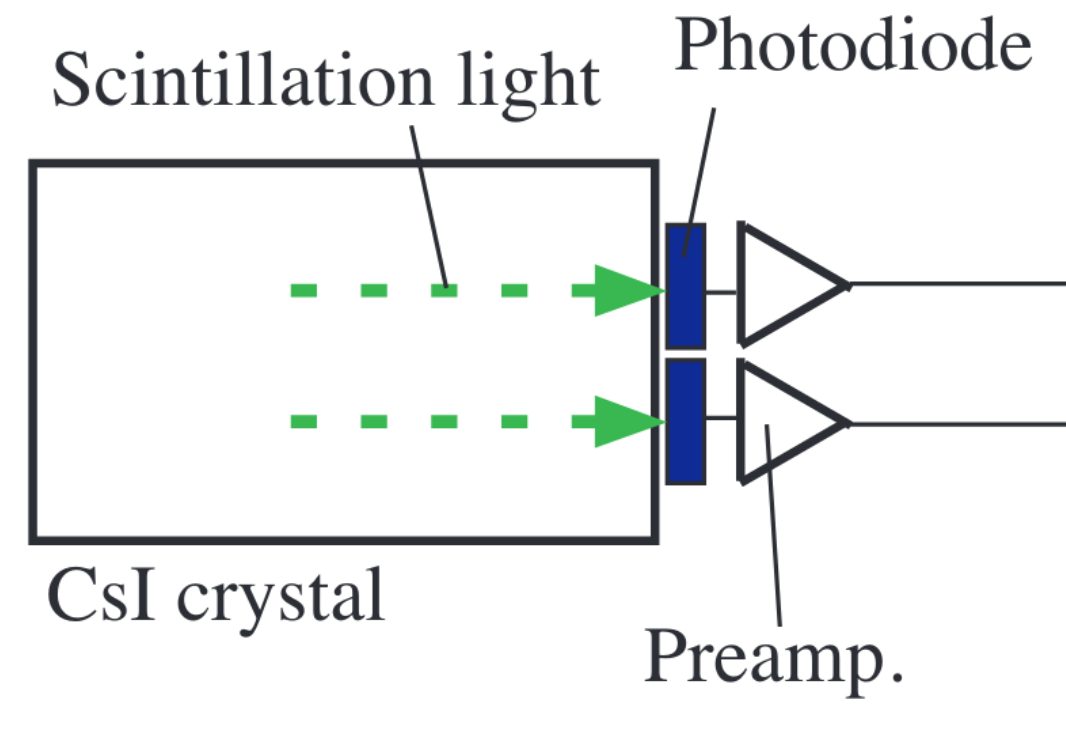
\includegraphics[width=0.45\textwidth]{figures/experimental_setup/ecl.png}
    \caption{\label{fig:ecl}
    A schematic depiction of one of the crystals that comprise the Belle~II electromagnetic calorimeter.
    A signal resulting from the shower of an electromagnetically interacting particle reaches the photodiode and is amplified by the preamplifier.
    Credit to Ref.~\cite{Miyabayashi:2020xzp}.
    }
\end{figure}

\subsection{Superconducting magnet}\label{sec:magnet}

Surrounding the \ECL \cite{Belle-II:2010dht}, there is the superconducting solenoid.
The coil is made from a niobium-titanium-copper alloy and is wound around an aluminium support cylinder.
The cooling is performed using a liquid helium cryogenic system.
It generates a $1.5~\mathrm{T}$ magnetic field necessary 
to bend the trajectories of charged particles, 
enabling a transverse momentum measurement and charge separation.
The magnetic field is directed along the $z$ direction 
and was measured to be homogeneous and vary less than $\order(1\%)$ in the entire volume \cite{BelleIITrackingGroup:2020hpx}.

\subsection{\texorpdfstring{$K_L^0$}{KL} and \texorpdfstring{\mu}{mu} detector}\label{sec:klm}

The $K_L^0$ and $\mu$ detector (\KLM) \cite{Aushev:2014spa} is the outermost subsystem of Belle~II.
The \KLM is composed of alternating layers of up to $4.7~\cm$ thick iron plates and detector active parts.
The iron plates decelerate the traversing particles and also act as a return yoke for the magnet.

The barrel and endcap regions differ by design \cite{Krohn:317929}.
The barrel region contains 14 iron layers and 15 detector layers, which are aligned parallel to the $z$ axis.
There, two innermost detector layers are instrumented with scintillator strips, 
whereas the remaining layers use resistive plate chambers.
The endcap region contains 14 iron and detector layers each, which are aligned perpendicular to the $z$ axis.
Conversely, all 14 detector layers use plastic silicon strips with silicon photomultipliers.

The $K_L^0$ mesons interact with the nuclei in the iron plates and cause hadronic showers, 
which are read out by the silicon strip detectors or the resistive plate chambers.
This process may already occur in the \ECL, which is why it is also a part of $K_L^0$ detection.
Minimum ionising particles, such as $\mu$ with momentum larger than 0.6~\gevc, traverse the detector in a straight line, 
depositing only small amounts of energy in the system.

\begin{figure}[htbp!]
    \subcaptionbox{\label{fig:rpc_klm}}{
        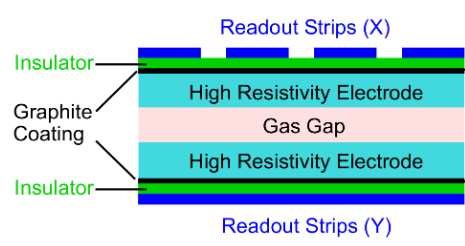
\includegraphics[width=0.45\textwidth]{figures/experimental_setup/rpc_klm.png}
    }
    \subcaptionbox{\label{fig:scintilator_klm}}{
        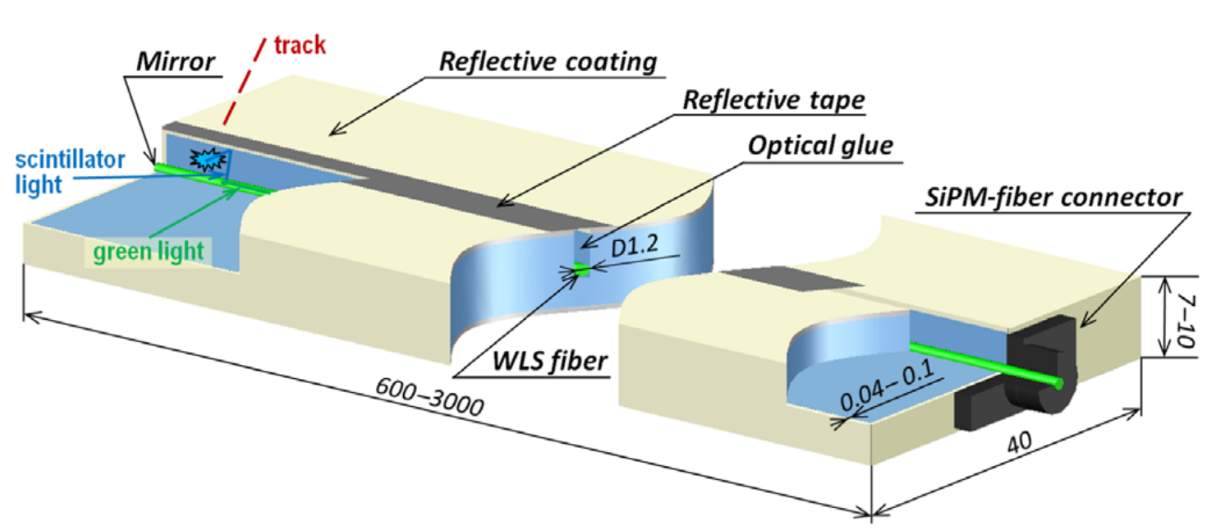
\includegraphics[width=0.45\textwidth]{figures/experimental_setup/scintilator_klm.png}
    }
    \caption{\label{fig:klm}
        The Belle~II $K_L^0$ and $\mu$ detector active detector layers in the barrel (\Cref{fig:rpc_klm}) and the endcap regions (\Cref{fig:scintilator_klm}).
        Iron plates are sandwiched between the detector layers.
        Credit to Refs.~\cite{Krohn:317929} and \cite{Aushev:2014spa}, respectively.
    }
\end{figure}

\section{The Belle II software}\label{sec:belle2_software}

The Belle~II analysis software (\basftwo) \cite{Kuhr:2018lps} is an open-source software framework developed for collision event reconstruction, analysis 
and any other tasks necessary for the physical interpretation of the data recorded by the Belle~II detector.
The software is primarily based on \texttt{Python} and \texttt{C++} programming languages.
This section briefly introduces the charged and neutral particle reconstruction strategies, which are implemented in \basftwo.

\subsection{Charged particle reconstruction}\label{sec:tracking}

Tracking refers to the charged particle trajectory reconstruction.
The tracking process in Belle~II is discussed broadly in Ref.\cite{BelleIITrackingGroup:2020hpx}.
Each particle trajectory is modelled by a helix with 5 parameters (track):
\begin{itemize}
    \item $d_0$: the distance of the point of the closest approach to the $z$ axis;
    \item $\phi_0$: the angle between the transverse momentum and the $x$ axis at the point of the closest approach;
    \item $\omega$: the track curvature signed with the particle charge;
    \item $z_0$: the $z$ coordinate at $d_0$;
    \item $\tan\lambda$: the tangent of the track dip angle (see \Cref{fig:sz_helix}).
\end{itemize}
These track parameters are visualised in \Cref{fig:helix}.
\begin{figure}[htbp!]
    \centering
    \subcaptionbox{\label{fig:xy_helix}}{
        \clipbox*{0 {0\height} {.32\width} {1\height}}{%
        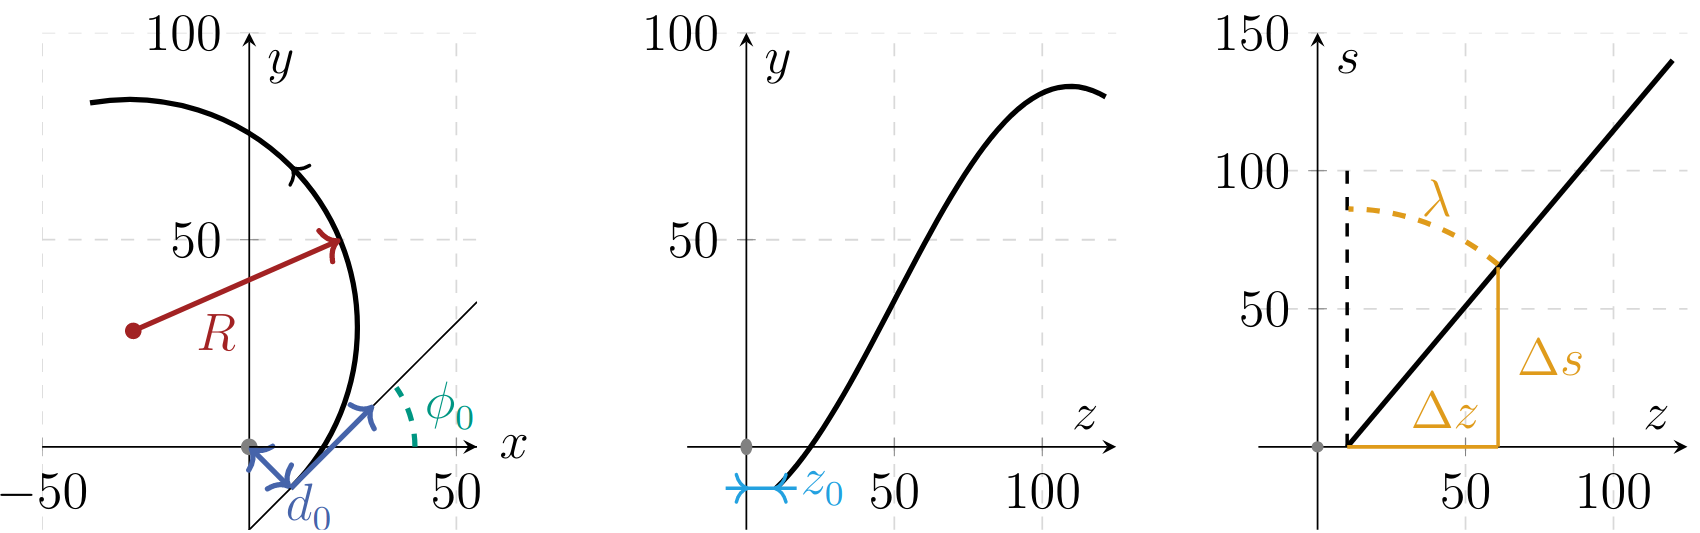
\includegraphics[width=0.95\textwidth]{figures/experimental_setup/helix.png}
        }
    }
    \subcaptionbox{\label{fig:yz_helix}}{
        \clipbox*{{.34\width}  {0\height} {.66\width} {1\height}}{%
        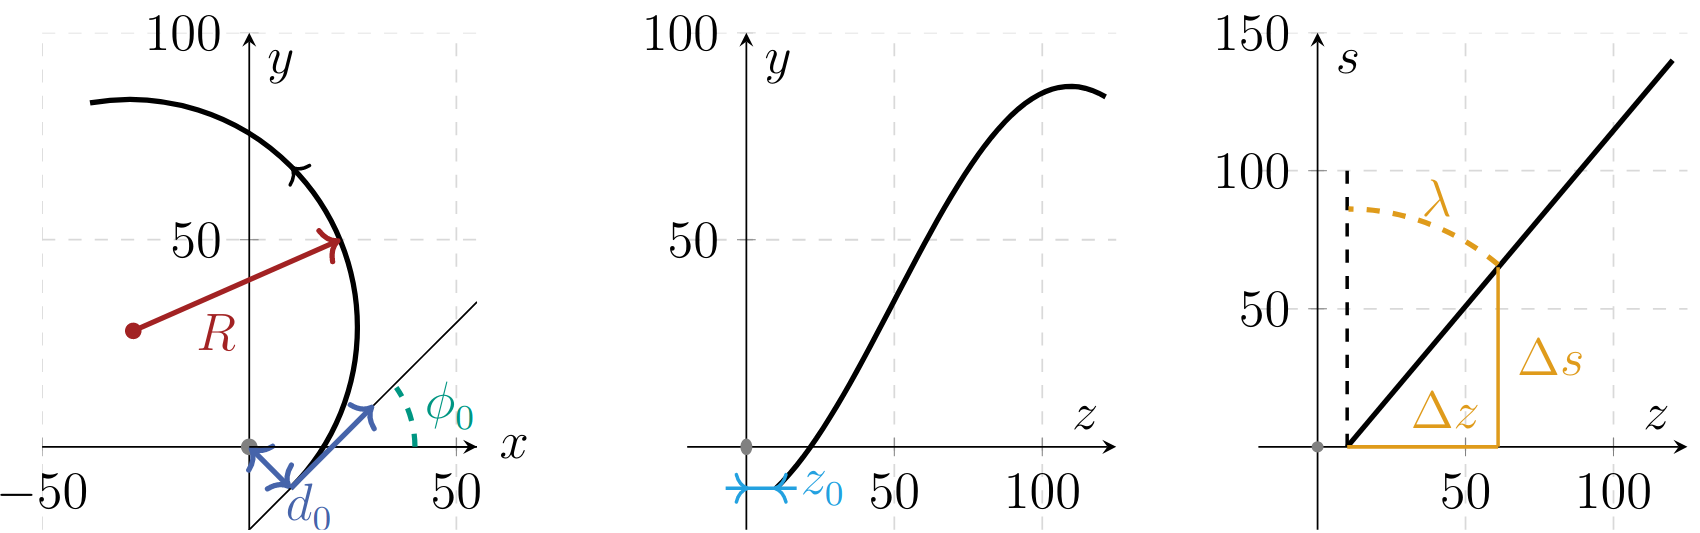
\includegraphics[width=0.95\textwidth]{figures/experimental_setup/helix.png}
        }
    }
    \subcaptionbox{\label{fig:sz_helix}}{
        \clipbox*{{.66\width} {0\height} {0.99\width} {1\height}}{%
        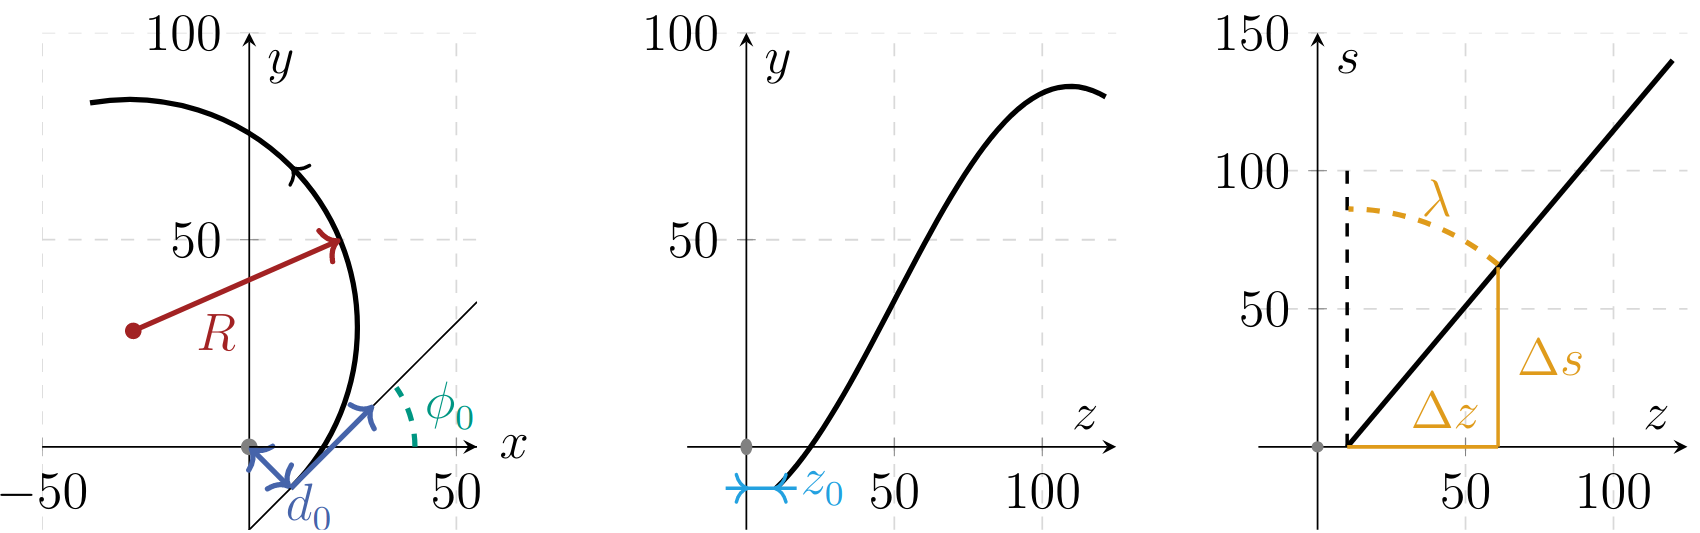
\includegraphics[width=0.95\textwidth]{figures/experimental_setup/helix.png}
        }
    }
    \caption{\label{fig:helix} A schematic representation of a track in Belle~II and the corresponding helix parameters that model it.
    All dimensions are in centimetres.
    In this context, $s$ corresponds to the path length along the circular trajectory in the $xy$ plane.
    The definition of the various helix parameters is given in \Cref{sec:tracking}.
    The Figures are taken from Ref.~\cite{BelleIITrackingGroup:2020hpx}.
    }
\end{figure}
The tracks are reconstructed by combining the information from \CDC and/or \SVD with information from \PXD, if present.

\subsection{Photon reconstruction}\label{sec:neutrals}

Particle showering in the \ECL material deposit energy into \ECL crystals.
The deposited energy and the time of each energy deposit are recorded by the calorimeter.
Clusters are sets of energy deposits in the \ECL that are associated with the interactions of a single particle.
A graphical illustration of the cluster reconstruction in an experimental environment is shown in \Cref{fig:clustering}.
\begin{figure}[htbp!]
    \centering
    \subcaptionbox{\label{fig:clustering1}}{
    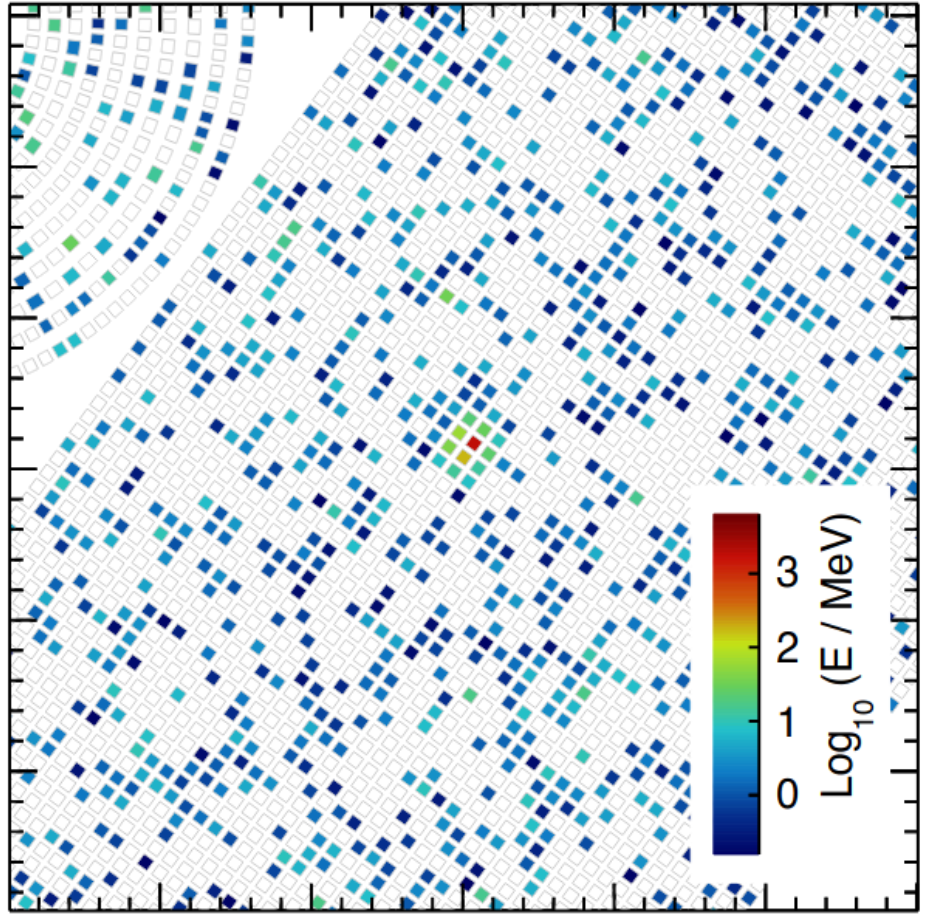
\includegraphics[width=0.4\textwidth]{figures/experimental_setup/clustering1.png}
    }
    \subcaptionbox{\label{fig:clustering2}}{
        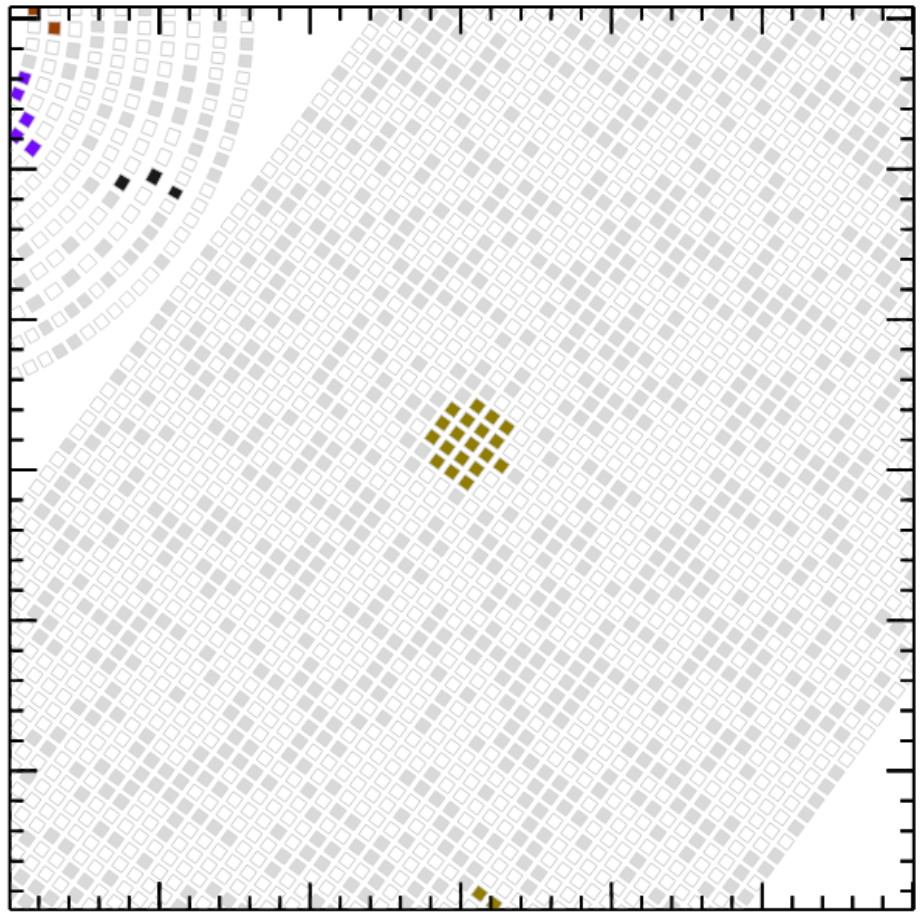
\includegraphics[width=0.4\textwidth]{figures/experimental_setup/clustering2.png}
    }
    \caption{\label{fig:clustering}
    The Belle~II calorimeter in the $\theta-\phi$ plane is visualised, 
    showcasing energy deposits in a single simulated photon event in the centre of the image.
    Each point corresponds to a single \ECL crystal.
    The low-energy deposits resulting from beam background radiation are included.
    The cluster reconstruction algorithm of \basftwo singles out the cluster from the photon, 
    rejecting background as seen in \Cref{fig:clustering2}.
    Credit to Belle~II Neutrals group.
    }
\end{figure}

The identification of photons exploits the fact that the energy deposited in the cluster
by an incident photon has a cylindrical symmetry in the lateral direction with an exponentially decreasing energy deposition away from the incident axis.
On the other hand, neutral or charged hadrons interactions tend to produce less confined and more asymmetric shower shapes.
To distinguish photons from charged particles (particularly electrons) tracks are extrapolated to the \ECL and compared for consistency with reconstructed clusters.
